% ZPD priekšvariants: veidne (../template/zpd.cls), aizpildīta ar šī projekta saturu.
% Sarkanās piezīmes paskaidro, kas ir katra daļa; [sarkanā iekavās] -- vēl jāaizpilda.
% Skaitļi tabulās un attēlos nāk no ../scripts/make_figures.py (results/ mapē).
% Kompilē: make preliminary  (no mapes zpd_darbs/)
\documentclass{../template/zpd}
\graphicspath{{../template/}{../figures/}}
\newcommand{\jgexTotal}{231}
\newcommand{\jgexSolved}{205}
\newcommand{\jgexBest}{217}
\newcommand{\jgexMedian}{1,9}
\newcommand{\imoSolved}{15}
\newcommand{\imoBest}{16}
\newcommand{\imoTotal}{29}
\newcommand{\auxBest}{7}
\newcommand{\auxTotal}{101}
\newcommand{\stuckSolved}{20}
\newcommand{\midOneAux}{5}

\newcommand{\modelParams}{2\,1}
\newcommand{\trainExamples}{98\,008}
\newcommand{\trainSteps}{1600}
\newcommand{\bestValLoss}{0,57}


\skola{RTU Inženierzinātņu vidusskola}
\nosaukums{Vieglu ģeometrijas risinājumu skeneris}
\nozaru{dabaszinātņu nozaru grupas datorzinātnes un informātikas nozarē}
\autors[Darba autors]{\aizpildit{Vārds Uzvārds}}
\vaditajs[Darba vadītājs]{\aizpildit{Vārds Uzvārds}}
\pilseta{Rīga}
\gads{2026}
\logotips{../template/logo_rtu_izv.png}

\begin{document}

\titullapa

% ==================================================================== anotācijas
\anotacijulapa
\begin{anotacija}{Anotācija}
\zpdlabel{Autors un nosaukums}\aizpildit{Vārds Uzvārds}. Vieglu ģeometrijas risinājumu skeneris.

\zpdlabel{Mērķis, metode, rezultāti}Darbā izstrādāts rīks, kas olimpiāžu ģeometrijas uzdevumu kopā
izvēlētai ģeometrijas jomai (likumu kopai) atrod uzdevumus ar vieglu risinājumu: tādu, kas pierādāms
tikai ar jomas likumiem, ne vairāk kā vienu palīgkonstrukciju, 60~s un 2~GB atmiņas. Rīks balstās uz
AlphaGeometry pieeju: determinēts DD-AR dzinējs (Newclid) pierāda faktus, bet palīgpunktus piedāvā
cilvēka heiristikas un paša apmācīts mazs transformeris. Definētas trīs jomas, katra ar algebrisko
spriešanu un bez tās. Uz \jgexTotal{} JGEX uzdevumiem DD-AR vienatnē atrisina \jgexSolved{},
vairāk nekā AlphaGeometry DD+AR (198); ar 5,1 milj. parametru transformeri, kas apmācīts 3,4 stundas
uz diviem CPU kodoliem, -- \jgexBest{}, un IMO-AG-30 etalonā \imoBest{} no \imoTotal{}. \aizpildit{Galvenie secinājumi pēc skenēšanas.}

\atslegvardi{automātiskā teorēmu pierādīšana, deduktīvā datubāze, palīgkonstrukcija, transformeris, olimpiāžu matemātika}
\end{anotacija}

\begin{anotacija}{Abstract}
\zpdlabel{Tulkojums angļu valodā}\aizpildit{Name Surname}. A Scanner for Easy Geometry Solutions.

The work develops a tool that, for a chosen geometry domain (a set of deduction rules), finds the
olympiad geometry problems that have an easy solution: one provable with the domain's rules only,
at most one auxiliary construction, 60~s and 2~GB of memory. It follows the AlphaGeometry approach:
a deterministic DD-AR engine (Newclid) proves facts, while auxiliary points come from human
heuristics and a small transformer trained from scratch. Three domains are defined, each with and
without algebraic reasoning. On \jgexTotal{} JGEX problems DD-AR alone solves \jgexSolved{}, more
than AlphaGeometry's DD+AR (198); with a 5.1M-parameter transformer trained for 3.4 hours on two CPU
cores it solves \jgexBest{}, and \imoBest{} of \imoTotal{} on the IMO-AG-30 benchmark. \aizpildit{Main conclusions after the scan.}

\atslegvardi[Keywords]{automated theorem proving, deductive database, auxiliary construction, transformer, olympiad mathematics}
\end{anotacija}

\saturs

% ==================================================================== ievads
\pamatteksts
\nenumuretanodala{Ievads}
\zpdlabel{Temata izvēles pamatojums}Olimpiāžu ģeometrijas uzdevumu krājumos grūtība parasti ir norādīta
subjektīvi, pēc autora vai žūrijas vērtējuma, un nav redzams, kuri uzdevumi patiesībā atrisināmi ar
vienas tēmas zināšanām. Skolotājiem un skolēniem būtu noderīgi zināt, kuri uzdevumi atrisināmi tikai
ar konkrētas jomas teorēmām, kuriem nepieciešama viena ,,atslēgas`` palīgkonstrukcija un kura tieši.

\zpdlabel{Problēma un aktualitāte}Ar roku šādu analīzi veikt simtiem uzdevumu ir lēni un neprecīzi.
AlphaGeometry tipa sistēmas \atsauce{Trinh u.c., 2024} ļauj to automatizēt, jo to pierādījumi ir
pārbaudāmi soli pa solim, un katra rīka ieguldījumu var kontrolēt atsevišķi. Šādu sistēmu mērķis
līdz šim ir bijis atrisināt pēc iespējas vairāk uzdevumu, nevis noteikt, cik viegls ir risinājums
noteiktā jomā.

\zpdlabel{Darba mērķis}Izveidot un pārbaudīt rīku, kas olimpiāžu ģeometrijas uzdevumu kopā izvēlētai
ģeometrijas jomai atrod uzdevumus ar vieglu risinājumu, parāda šos risinājumus un izmērāmi raksturo
to vieglumu.

\zpdlabel{Darba uzdevumi}
\begin{enumerate}
  \item Izveidot risinātāju, kas apvieno DD-AR dzinēju ar palīgpunktu avotiem un darbojas
        dotajos laika un atmiņas resursos.
  \item Definēt ģeometrijas jomas kā likumu kopas un ,,viegla risinājuma`` iestatījumu.
  \item Apmācīt transformeri palīgpunktu piedāvāšanai un novērtēt tā piedāvājumu derīgumu.
  \item Savākt un pārtulkot Newclid sintaksē Latvijas olimpiāžu ģeometrijas uzdevumus un
        noskenēt tos visās jomās.
  \item Salīdzināt jomas un palīgpunktu avotus un atrastos vieglos risinājumus ar oficiālo grūtību.
\end{enumerate}

\zpdlabel{Hipotēze}Daļai olimpiāžu ģeometrijas uzdevumu eksistē viegls risinājums vienā šaurā jomā
(piemēram, tikai ar riņķa līnijām un ievilktajiem leņķiem), un šādi uzdevumi biežāk ir zemākas
oficiālās grūtības uzdevumi.

\zpdlabel{Pētījuma metodes}Modelēšana (DD-AR deduktīvā spriešana un transformera modelis),
eksperiments (uzdevumu skenēšana dažādās jomās un ar dažādiem palīgpunktu avotiem), salīdzināšana
un statistiskā analīze.

% ==================================================================== 1. nodaļa
\section{Ģeometrijas uzdevumu automātiskā risināšana}
\zpdnote{Literatūras apskats: ne vairāk kā 1/3 no darba teksta.}
\subsection{Deduktīvās datubāzes metode}
Deduktīvās datubāzes (DD) metode \atsauce{Chou u.c., 2000} no uzdevuma pieņēmumiem atkārtoti
pielieto ģeometrijas likumus (piemēram, ,,ja četri punkti atrodas uz vienas riņķa līnijas, tad
ievilktie leņķi ir vienādi``), līdz jauni fakti vairs nerodas. Algebriskā spriešana (AR) to papildina
ar leņķu un attiecību vienādojumu risināšanu. Kopā tās veido DD-AR, kas pierāda faktus bez kļūdām,
bet nevar ieviest jaunus punktus. Darbā izmantota atvērtā pirmkoda Newclid realizācija
\atsauce{Sicca u.c., 2024}. \aizpildit{Kritisks salīdzinājums ar Wu metodi un Gröbnera bāzēm.}

\subsection{Valodas modeļi palīgkonstrukcijām}
AlphaGeometry \atsauce{Trinh u.c., 2024} parādīja, ka transformeris \atsauce{Vaswani u.c., 2017},
apmācīts uz sintētiskiem pierādījumiem, var piedāvāt palīgpunktus, kas DD-AR ļauj pabeigt
pierādījumu; AlphaGeometry2 \atsauce{Chervonyi u.c., 2025} sasniedza zelta medaļas līmeni
IMO uzdevumos. Abu sistēmu modeļi ir lieli un apmācīti uz GPU. GenesisGeo \atsauce{Zhu u.c., 2025}
publicēja atvērtu sintētisku datu kopu, kas ļauj apmācīt mazu modeli uz CPU.
\aizpildit{Salīdzinājums: ko šie darbi mēra un ko nemēra (risinājuma vieglumu).}

\zpdlabel{Nodaļas kopsavilkums}DD-AR dod pārbaudāmus pierādījumus, bet tam vajag palīgpunktus no
ārpuses. Neviens no apskatītajiem darbiem nemēra, vai risinājums ir viegls noteiktā likumu kopā;
to dara šis darbs.

% ==================================================================== 2. nodaļa
\section{Metodes}
\subsection{Risinātājs}
Risinātājs vispirms palaiž DD-AR uz uzdevuma; ja mērķis netiek pierādīts, palīgpunktu avoti piedāvā
punktus, katrs tiek pievienots un DD-AR tiek palaists vēlreiz. Viss izsaukums notiek atsevišķā
procesā ar laika, atmiņas un CPU ierobežojumiem, un rezultātā tiek saglabāts pierādījums,
palīgkonstrukcija, izmantotie likumi un patērētie resursi.

\subsection{Jomas un viegla risinājuma definīcija}
Joma ir DD-AR likumu kopa ar AR vai bez tā. Definētas trīs jomas: \texttt{full} (70 likumi),
\texttt{circles} (29 likumi: riņķa līnijas un ievilktie leņķi) un \texttt{no\_similarity}
(59 likumi: \texttt{full} bez līdzīgajiem trijstūriem). Risinājums ir viegls jomā $J$, ja
\begin{equation}
  \text{likumi} \subseteq J, \qquad \text{dziļums} \le 1, \qquad t \le 60~\text{s}, \qquad m \le 2~\text{GB}.
  \label{eq:viegls}
\end{equation}

\subsection{Transformeris un dati}
No nulles uzrakstīts transformeris \atsauce{Vaswani u.c., 2017} (GPT tipa dekoderis, PyTorch
\atsauce{Paszke u.c., 2019}) apmācīts uz \trainExamples{} GenesisGeo piemēriem: uzdevuma
pieņēmumi un mērķis $\to$ palīgpunkts. Apmācīti trīs modeļi uz 2 CPU kodoliem: \texttt{mini}
(2,1 milj. parametru, 1600 soļi), tas pats modelis ilgāk (\texttt{mini\_long}, 9000 soļi) un
lielāks \texttt{mid} (5,1 milj. parametru, 6 slāņi, 9000 soļi). Modeļa piedāvājumi tiek pārvērsti
Newclid konstrukcijās; tos, kas neatbilst zīmējumam, risinātājs atmet.

Salīdzinājumam sagatavoti arī gatavi modeļi: GenesisGeo \atsauce{Zhu u.c., 2025}, AlphaGeometry
valodas modelis \atsauce{Trinh u.c., 2024} un mazi vispārīgi valodas modeļi.
\aizpildit{Salīdzinājuma rezultāti (8.4. uzdevums): kurš modelis jomā visātrāk atrod vienu palīgpunktu.}

\subsection{Uzdevumu kopa}
No Neklātienes matemātikas skolas arhīva savākti 6333 Latvijas olimpiāžu uzdevumi, no tiem 1499
ģeometrijā. \aizpildit{Darba kopas izvēle, tulkošana un skaitliskā pārbaude (7.2.--7.6. uzdevums).}

% ==================================================================== 3. nodaļa
\section{Rezultāti un analīze}
\zpdnote{Priekšvarianta rezultāti: parauga uzdevumi un JGEX. Latvijas uzdevumu skenēšana vēl nav veikta.}
\subsection{Jomas uz parauga uzdevumiem}
Uz pieciem parauga uzdevumiem jomas atšķir uzdevumus, kā gaidīts (\ref{tab:domains}~tabula,
\ref{fig:domains}~attēls): Varinjona teorēmai vajag viduslīnijas teorēmu, kas nav riņķa līniju
teorēma, un bez AR izkrīt uzdevumi, kuros vajag leņķu skaitīšanu.

\begin{table}[H]
  \caption{Parauga uzdevumu atrisināšana sešās jomās (60~s, 2~GB, dziļums $\le 1$)}\label{tab:domains}
  \centering\small
  \begin{tabular}{@{}l*{6}{c}@{}}
    \toprule
    Uzdevums & \texttt{full} & bez AR & \texttt{circles} & bez AR & \texttt{no\_sim.} & bez AR \\
    \midrule
    \csname @@input\endcsname ../tables/domains_examples.tex 
    \bottomrule
  \end{tabular}\\[3pt]
  {\footnotesize nē (laiks) -- 60~s limits; nē (dziļ.) -- nav atrisināts ar $\le 1$ palīgpunktu; nē (zīm.) -- zīmējumu nevar izveidot (nepareizs tulkojums).}
\end{table}

\begin{figure}[H]
  \centering
  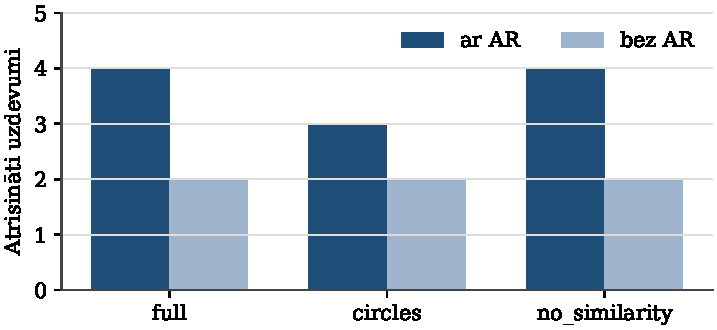
\includegraphics[width=0.8\textwidth]{domains_examples.pdf}
  \caption{Atrisināto parauga uzdevumu skaits katrā jomā ar AR un bez tā}\label{fig:domains}
\end{figure}

\subsection{Standarta uzdevumu kopas}
Risinātājs pārbaudīts uz trim Newclid publicētām kopām ar 60~s un 2~GB uz uzdevumu
(\ref{tab:bench}~tabula). DD-AR vienatnē atrisina \jgexSolved{} no \jgexTotal{} JGEX uzdevumiem
(mediāna \jgexMedian~s) un \imoSolved{} no \imoTotal{} IMO-AG-30 uzdevumiem, vairāk nekā
AlphaGeometry DD+AR \atsauce{Trinh u.c., 2024}. Modeļi palaisti tikai uzdevumos, kuros DD-AR
iestrēgst (ar līdz diviem palīgpunktu līmeņiem).

\begin{table}[H]
  \caption{Atrisināto uzdevumu skaits standarta kopās; AlphaGeometry skaitļi no \atsauce{Trinh u.c., 2024}}\label{tab:bench}
  \centering\small
  \begin{tabular}{@{}lccccccc@{}}
    \toprule
    & & & \multicolumn{3}{c}{Šis darbs} & \multicolumn{2}{c}{AlphaGeometry} \\
    \cmidrule(lr){4-6}\cmidrule(l){7-8}
    Kopa & Uzd. & DD-AR & + \texttt{mini\_long} & + \texttt{mid} & Kopā & DD+AR & ar modeli \\
    \midrule
    \csname @@input\endcsname ../tables/bench.tex 
    \bottomrule
  \end{tabular}\\[3pt]
  {\footnotesize IMO-AG-30: 29 no 30 uzdevumiem (Newclid kopā trūkst \texttt{2000\_p1}).
  IMO, vajag palīgpunktu: uzdevumi, ko Newclid DD-AR vienatnē neatrisina.}
\end{table}

Modeļi atrisina \stuckSolved{} uzdevumus, kuros DD-AR iestrēgst (\ref{tab:solved}~tabula);
\texttt{mid} pirmo reizi pievieno IMO-AG-30 uzdevumu (2015.~gada 3.~uzdevums). Vieglā risinājuma
definīcijai (viens palīgpunkts) atbilst \midOneAux{} no \texttt{mid} risinājumiem. Laika limits
netika sasniegts nevienā uzdevumā: ierobežo piedāvājumu kvalitāte, nevis laiks.

\begin{table}[H]
  \caption{Uzdevumi, kuros DD-AR vienatnē iestrēgst, bet modelis atrod pierādījumu: palīgpunktu skaits (p.) un laiks}\label{tab:solved}
  \centering\small
  \begin{tabular}{@{}llcc@{}}
    \toprule
    Kopa & Uzdevums & \texttt{mini\_long} & \texttt{mid} \\
    \midrule
    \csname @@input\endcsname ../tables/bench_solved.tex 
    \bottomrule
  \end{tabular}
\end{table}

\subsection{Transformera novērtējums}
Uz \evalProblems{} neredzētiem GenesisGeo uzdevumiem (\ref{tab:models}~tabula) ap 90~\% piedāvājumu
ir pārvēršami Newclid konstrukcijās visiem modeļiem, bet precīza sakritība ar atsauces palīgpunktu
aug ar apmācības ilgumu un modeļa izmēru: no 21~\% līdz 53,5~\%, ja skaita jebkuru no četriem
piedāvājumiem. Validācijas zudums lielākajam modelim ir zemāks katrā apmācības solī
(\ref{fig:training}~attēls).

\begin{table}[H]
  \caption{Apmācītie modeļi un to piedāvājumi uz \evalProblems{} neredzētiem uzdevumiem (staru meklēšana, 4 stari)}\label{tab:models}
  \centering\small
  \begin{tabular}{@{}lccccccc@{}}
    \toprule
    Modelis & Milj. param. & Soļi & Laiks & Val. zudums & Pārvēršami & Precīzi, 1. & Precīzi, 4 \\
    \midrule
    \csname @@input\endcsname ../tables/training_models.tex 
    \bottomrule
  \end{tabular}
\end{table}

\begin{figure}[H]
  \centering
  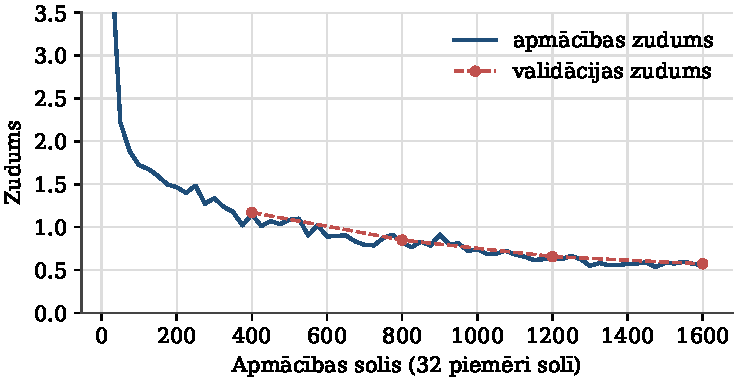
\includegraphics[width=0.8\textwidth]{training_loss.pdf}
  \caption{Validācijas zudums apmācības laikā uz 2 CPU kodoliem}\label{fig:training}
\end{figure}

\zpdlabel{Nodaļas kopsavilkums}\aizpildit{Pēc Latvijas uzdevumu skenēšanas: cik uzdevumu katrā jomā ir viegli, kuras teorēmas tos padara vieglus, salīdzinājums ar oficiālo grūtību.}

% ==================================================================== secinājumi
\nenumuretanodala{Secinājumi}
\zpdnote{Priekšvarianta secinājumi; galīgajā darbā -- ne vairāk kā uzdevumu (5), katrs atbilst uzdevumam.}
\begin{secinajumi}
  \item Risinātājs DD-AR + palīgpunkti darbojas uz CPU 60~s un 2~GB budžetā; DD-AR vienatnē
        atrisina \jgexSolved{} no \jgexTotal{} JGEX uzdevumiem, vairāk nekā AlphaGeometry DD+AR.
  \item Jomas kā likumu kopas atšķir uzdevumus: šaurākā \texttt{circles} jomā atrisināti 3 no 5
        parauga uzdevumiem, \texttt{full} jomā -- 4 no 5.
  \item Uz CPU apmācīts mazs transformeris piedāvā derīgas konstrukcijas (ap 90~\%) un atrisina
        \stuckSolved{} uzdevumus, kuros DD-AR iestrēgst, arī vienu IMO-AG-30 uzdevumu; lielāks modelis
        palīdz nedaudz vairāk, un to ierobežo piedāvājumu kvalitāte, nevis laiks.
  \item \aizpildit{Secinājums par Latvijas uzdevumu skenēšanu.}
  \item \aizpildit{Secinājums par saistību ar oficiālo grūtību (hipotēzes pārbaude).}
\end{secinajumi}

% ==================================================================== avoti
\begin{avoti}
  \avots Chervonyi, Y., Trinh, T. H., Olšák, M. u.c. (2025). \textit{Gold-medalist Performance in Solving Olympiad Geometry with AlphaGeometry2} [tiešsaiste]. arXiv:2502.03544 [skatīts 2026. gada 5. novembrī]. Pieejams: \url{https://arxiv.org/abs/2502.03544}
  \avots Chou, S.-C., Gao, X.-S., Zhang, J.-Z. (2000). A Deductive Database Approach to Automated Geometry Theorem Proving and Discovering. \textit{Journal of Automated Reasoning}, Vol. 25, pp. 219--246.
  \avots Paszke, A. u.c. (2019). PyTorch: An Imperative Style, High-Performance Deep Learning Library. \textit{Advances in Neural Information Processing Systems 32 (NeurIPS 2019)}, pp. 8024--8035.
  \avots Sicca, V. u.c. (2024). \textit{Newclid: A User-Friendly Replacement for AlphaGeometry} [tiešsaiste]. arXiv:2411.11938 [skatīts 2026. gada 5. novembrī]. Pieejams: \url{https://arxiv.org/abs/2411.11938}
  \avots Trinh, T. H., Wu, Y., Le, Q. V., He, H., Luong, T. (2024). Solving olympiad geometry without human demonstrations. \textit{Nature}, Vol. 625, pp. 476--482.
  \avots Vaswani, A., Shazeer, N., Parmar, N. u.c. (2017). Attention Is All You Need. \textit{Advances in Neural Information Processing Systems 30 (NIPS 2017)}, pp. 5998--6008.
  \avots Zhu, M., Wang, Z. u.c. (2025). \textit{GenesisGeo: Technical Report} [tiešsaiste]. arXiv:2509.21896 [skatīts 2026. gada 5. novembrī]. Pieejams: \url{https://arxiv.org/abs/2509.21896}
  \avots \textit{Olimpiāžu uzdevumu arhīvs} [tiešsaiste]. LU Neklātienes matemātikas skola [skatīts 2026. gada 4. novembrī]. Pieejams: \url{https://www.nms.lu.lv/arhivs-un-materali/uzdevumu-arhivs/}
  \avots \aizpildit{Izmantotie mākslīgā intelekta rīki, ja tādi lietoti: Izstrādātājs. (Gads, datums). \textit{Rīks, versija un sarunas nosaukums} [tiešsaiste]. [skatīts ...]. Pieejams: ... (vadlīnijas, 1.2. un 5. pielikums)}
\end{avoti}

% ==================================================================== pielikumi
\pielikums{Uzdevuma pieraksts Newclid sintaksē}
\zpdnote{Piemērs, kā olimpiāžu uzdevums tiek pārtulkots (sk. docs/translation\_guide.md).}
{\footnotesize\begin{verbatim}
a b c = triangle a b c; h = orthocenter h a b c; d = reflect d h b c ? cyclic a b c d
\end{verbatim}}
Trijstūra $ABC$ ortocentra $H$ atspoguļojums pāri $BC$ atrodas uz $ABC$ apvilktās riņķa līnijas.

\end{document}
